\documentclass[12pt]{article}
\usepackage[margin=2.5cm]{geometry}
\usepackage{enumerate}
\usepackage{amsfonts}
\usepackage{amsmath}
\usepackage{fancyhdr}
\usepackage{amsmath}
\usepackage{amssymb}
\usepackage{amsthm}
\usepackage{mdframed}
\usepackage{graphicx}
\usepackage{subcaption}
\usepackage{adjustbox}
\usepackage{listings}
\usepackage{xcolor}
\usepackage{booktabs}
\usepackage[utf]{kotex}
\usepackage{hyperref}
\usepackage{accents}

\definecolor{codegreen}{rgb}{0,0.6,0}
\definecolor{codegray}{rgb}{0.5,0.5,0.5}
\definecolor{codepurple}{rgb}{0.58,0,0.82}
\definecolor{backcolour}{rgb}{0.95,0.95,0.92}

\lstdefinestyle{mystyle}{
    backgroundcolor=\color{backcolour},
    commentstyle=\color{codegreen},
    keywordstyle=\color{magenta},
    numberstyle=\tiny\color{codegray},
    stringstyle=\color{codepurple},
    basicstyle=\ttfamily\footnotesize,
    breakatwhitespace=false,
    breaklines=true,
    captionpos=b,
    keepspaces=true,
    numbers=left,
    numbersep=5pt,
    showspaces=false,
    showstringspaces=false,
    showtabs=false,
    tabsize=1
}

\lstset{style=mystyle}

\pagestyle{fancy}
\renewcommand{\headrulewidth}{0.4pt}
\lhead{CSC 343}
\rhead{Worksheet 5}

\begin{document}
\title{CSC343 Worksheet 5}
\maketitle

\begin{enumerate}[1.]
    \item \textbf{Exercise 7.1.1:} Our running example movie database of Section
    2.2.8 has keys defined for all its relations.

    \begin{lstlisting}[language=SQL]
    Movies(title, year, length, genre, studioName, producerC#)
    Starsln(movieTitle, movieYear, starName)
    MovieStar(name, address, gender, birthdate)
    MovieExec(name, address, cert#, netWorth)
    Studio(name, address, presC#)
    \end{lstlisting}

    \bigskip

    Declare the following referential integrity constraints for the movie database as
    in Exercise 7.1.1.

    \begin{enumerate}[a)]
        \item The producer of a movie must be someone mentioned in MovieExec. Modifications to MovieExec that violate this constraint are rejected.
        \item Repeat (a), but violations result in the producerC\# in Movie being set to NULL.
        \item Repeat (a), but violations result in the deletion or update of the offending Movie tuple.
        \item A movie that appears in Stars ln must also appear in Movie. Handle violations by rejecting the modification.
        \item A star appearing in Stars ln must also appear in MovieStar. Handle violations by deleting violating tuples.
    \end{enumerate}

    \item \textbf{Exercise 7.1.2:} We would like to declare the constraint that every movie in
    the relation Movie must appear with at least one star in StarsIn. Can we do
    so with a foreign-key constraint? Why or why not?

    \item \textbf{Exercise 7.1.3:} Suggest suitable keys and foreign keys for the relations of the
    PC database:

    \begin{lstlisting}[language=SQL]
    Product(maker, model, type)
    PC(model, speed, ram, hd, price)
    Laptop(model, speed, ram, hd, screen, price)
    Printer(model, color, type, price)
    \end{lstlisting}

    \bigskip

    of Exercise 2.4.1. Modify your SQL schema from Exercise 2.3.1 to include
    declarations of these keys.

    \item \textbf{Exercise 7.1.4:} Suggest suitable keys for the relations of the battleships
    database

    \bigskip

    \begin{lstlisting}[language=SQL]
    Classes(class, type, country, numGuns, bore, displacement)
    Ships(name, class, launched)
    Battles(name, date)
    Outcomes(ship, battle, result)
    \end{lstlisting}

    \bigskip

    of Exercise 2.4.3. Modify your SQL schema from Exercise 2.3.2 to include
    declarations of these keys.

    \item \textbf{Exercise 7.1.5:} Exercise 7.1.5: Write the following referential
    integrity constraints for the battleships database as in Exercise 7.1.4. Use
    your assumptions about keys from that exercise, and handle all violations by
    setting the referencing attribute value to NULL

    \begin{enumerate}[a)]
        \item Every class mentioned in \textbf{Ships} must be mentioned in \textbf{Classes}.
        \item Every battle mentioned in \textbf{Outcomes} must be mentioned in \textbf{Battles}.
        \item Every ship mentioned in \textbf{Outcomes} must be mentioned in \textbf{Ships}.
    \end{enumerate}

    \item \textbf{Exercise 7.2.1:} Write the following constraints for attributes of the relation

    \begin{lstlisting}[language=SQL]
    Movies(title, year, length, genre, studioName, producerC#)
    \end{lstlisting}

    \bigskip

    \begin{enumerate}[a)]
        \item The year cannot be before 1915.
        \item The length cannot be less than 60 nor more than 250.
        \item The studio name can only be Disney, Fox, MGM, or Paramount.
    \end{enumerate}

    \item \textbf{Exercise 7.2.2:} Write the following constraints on attributes from our example
    schema

    \begin{lstlisting}[language=SQL]
    Product(maker, model, type)
    PC(model, speed, ram, hd, price)
    Laptop(model, speed, ram, hd, screen, price)
    Printer(model, color, type, price)
    \end{lstlisting}

    \bigskip

    of Exercise 2.4.1.

    \bigskip

    \begin{enumerate}[a)]
        \item The speed of a laptop must be at least 2.0.
        \item The only types of printers are laser, ink-jet, and bubble-jet.
        \item The only types of products are PC’s, laptops, and printers.
        \item A model of a product must also be the model of a PC, a laptop, or a printer.
    \end{enumerate}

    \item \textbf{Exercise 7.2.3:} Write the following constraints as tuple-based CHECK constraints
    on one of the relations of our running movies example:

    \begin{lstlisting}[language=SQL]
    Movies(title, year, length, genre, studioName, producerC#)
    Starsln(movieTitle, movieYear, starName)
    MovieStar(name, address, gender, birthdate)
    MovieExec(name, address, cert#, netWorth)
    Studio(name, address, presC#)
    \end{lstlisting}

    \bigskip

    If the constraint actually involves two relations, then you should put constraints
    in both relations so that whichever relation changes, the constraint will be
    checked on insertions and updates. Assume no deletions; it is not always possible
    to maintain tuple-based constraints in the face of deletions.

    \bigskip

    \begin{enumerate}[a)]
        \item A star may not appear in a movie made before they were born.
        \item No two studios may have the same address.
        \item A name that appears in \textbf{MovieStar} must not also appear in \textbf{MovieExec}.
        \item A studio name that appears in \textbf{Studio} must also appear in at least one \textbf{Movies} tuple.
    \end{enumerate}

    \item \textbf{Exercise 7.2.4:} Write the following as tuple-based CHECK constraints about
    our 'PC' schema.

    \bigskip

    \begin{enumerate}[a)]
        \item A PC with a processor speed less than 2.0 must not sell for more than \$600.
        \item A laptop with a screen size less than 15 inches must have at least a 40 gigabyte hard disk or sell for less than \$1000.
    \end{enumerate}

    \item \textbf{Exercise 7.2.5:} Write the following as tuple-based CHECK constraints about
    our 'battleships' schema:

    \bigskip

    \begin{lstlisting}[language=SQL]
    Classes(class, type, country, numGuns, bore, displacement)
    Ships(name, class, launched)
    Battles(name, date)
    Outcomes(ship, battle, result)
    \end{lstlisting}

    \begin{enumerate}[a)]
        \item No class of ships may have guns with larger than a 16-inch bore.
        \item If a class of ships has more than 9 guns, then their bore must be no larger than 14 inches.
        \item No ship can be in battle before it is launched.
    \end{enumerate}

    \item \textbf{Exercise 7.2.6:} In Examples 7.6 and 7.8, we introduced constraints on the
    gender attribute of \textbf{MovieStar}. What restrictions, if any, do each of these constraints
    enforce if the value of gender is NULL?

    \item \textbf{Exercise 7.3.1:} E xercise 7.3.1: Show how to alter your relation
    schemas for the movie example:

    \bigskip

    \begin{lstlisting}[language=SQL]
    Movies(title, year, length, genre, studioName, producerC#)
    Starsln(movieTitle, movieYear, starName)
    MovieStar(name, address, gender, birthdate)
    MovieExec(name, address, cert#, netWorth)
    Studio(name, address, presC#)
    \end{lstlisting}

    \bigskip

    in the following ways.

    \bigskip

    \begin{enumerate}[a)]
        \item Make title and year the key for \textbf{Movie}.
        \item Require the referential integrity constraint that the producer of every movie appear in \textbf{MovieExec}.
        \item Require that no movie length be less than 60 nor greater than 250.
        \item Require that no name appear as both a movie star and movie executive (this constraint need not be maintained in the face of deletions).
        \item Require that no two studios have the same address.
    \end{enumerate}

    \item \textbf{Exercise 7.3.2:} Show how to alter the schemas of the “battleships”
    database:

    \bigskip

    \begin{lstlisting}[language=SQL]
    Classes(class, type, country, numGuns, bore, displacement)
    Ships(name, class, launched)
    Battles(name, date)
    Outcomes(ship, battle, result)
    \end{lstlisting}

    \bigskip

    to have the following tuple-based constraints.

    \bigskip

    \begin{enumerate}[a)]
        \item \textbf{Class} and country form a key for relation \textbf{Classes}.
        \item Require the referential integrity constraint that every battle appearing in \textbf{Outcomes} also appears in \textbf{Battles}.
        \item Require the referential integrity constraint that every ship appearing in \textbf{Outcomes} appears in \textbf{Ships}.
        \item Require that no ship has more than 14 guns.
        \item Disallow a ship being in battle before it is launched.
    \end{enumerate}

    \item \textbf{Exercise 7.4.1:} Write the following assertions. The database schema is from
    the 'PC' example of Exercise 2.4.1:


    \begin{lstlisting}[language=SQL]
    Product(maker, model, type)
    PC(model, speed, ram, hd, price)
    Laptop(model, speed, ram, hd, screen, price)
    Printer(model, color, type, price)
    \end{lstlisting}

    \bigskip

    \begin{enumerate}[a)]
        \item No manufacturer of PC's may also make laptops.

        \begin{center}
        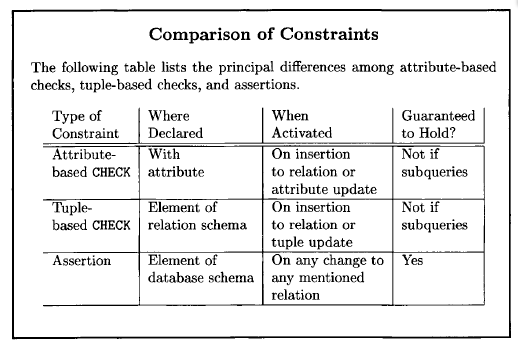
\includegraphics[width=0.7\linewidth]{images/worksheet_5_1.png}
        \end{center}
    \end{enumerate}


\end{enumerate}

\end{document}